\documentclass{beamer}
\usetheme{Warsaw}
\usepackage{hyperref}
\usepackage{amsmath}
\newcommand{\argmax}{\operatornamewithlimits{argmax}}

\title{Parsing Natural Scenes and Natural Language with Recursive Neural Networks}
\author{Seungwoo Yoo}
\date{\today}

\begin{document}
\frame{\titlepage}

\section[Outline]{}
\frame{\tableofcontents}

\section{Introduction}
\subsection{Recursive structure}
\frame
{
  \frametitle{Parsing Natural Structural Examples}
  \begin{columns}
  \column{0.5\textwidth}
  \begin{figure}[ht]  
	  \begin{center}
		  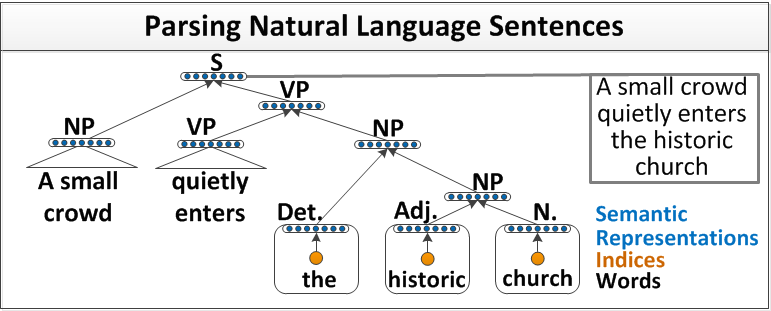
\includegraphics[width=2.1in]{images/fig1.png}   
	  \end{center}   
  \end{figure}
  \column{0.5\textwidth} 
  \begin{figure}[ht]
	  \begin{center}
		  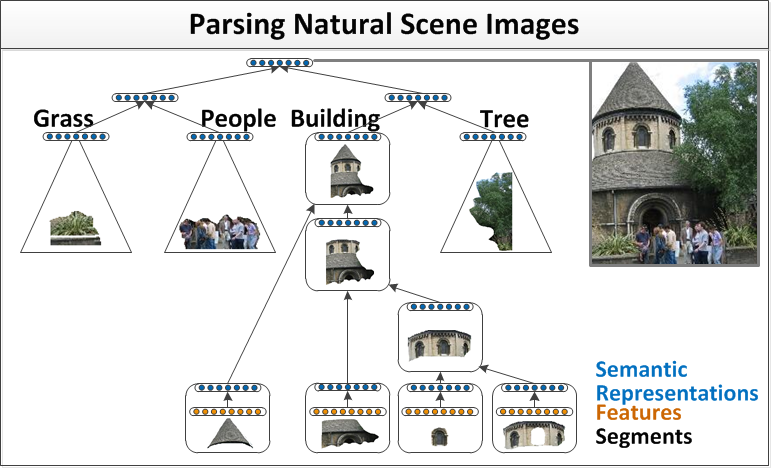
\includegraphics[width=2.1in]{images/fig2.png} 
	  \end{center}
  \end{figure}
  \end{columns}
  \begin{itemize}
  \item Ilustration of recursive neural network architectures
	\begin{enumerate}
	\item Segment features and word indices are mapped into semantic feature space
	\item Recursively merged by the same NN until they represent the entire image or sentence
	\end{enumerate}
  \end{itemize}
}
\frame
{
	\frametitle{Contributions}
	\begin{itemize}
		\item RNN can compute (for scene parsing):
			\begin{enumerate}
			\item a score that is higher when neighboring regions should be merged int a larger region
			\item a new semantic feature representation for this larger region and its class labels (e.g., \textit{building} or \textit{street})
			\end{enumerate}
		\item Contribution points
			\begin{itemize}
			\item First deep learning method to achieve state-of-the-art results on segmentation and annotations of complex scenes. 
			\item For scene classification, learned features outperfor state of the art methos such as Gist descriptor 
			\item Code for the RNN model is available at \url{http://www.socher.org}
			\end{itemize}
	\end{itemize}
}
\section{Algorithm Details}
\subsection{Mapping Segments and Words into Syntactico-Semantic Space}
\frame
{
	\frametitle{Input Representation of Scene Images}
	\begin{itemize}
		\item Feature extraction
			\begin{enumerate}
				\item Oversegment an image \textit{x} into superpixels using Meanshift algo. (only choose one set of parameters)
					\begin{itemize}
					\item This results in an average of 78 segments per image. 
					\end{itemize}
				\item Compute 119 dim features for the segments (same as \textit{Gould ICCV 2009} - color, texture, appearance, shape  features and boosted pixel classifier scores).
				\item Use a simple neural network layer to map these features into "semantic" \textit{n}-dim feature space :
				$$ a_i = f(W^{\textit{sem}}F_i+b^{sem}) $$ 
				$$ s.t., W^{sem} \in \mathbb{R}^{n\times119} \;and\; f(x)=1/(1+e^{-x})$$
			\end{enumerate}
	\end{itemize}
}
\frame
{
	\frametitle{Input Representation of Natural Language Sentences}
	\begin{itemize}
		\item Use a neural language models
		$$ a_i = Le_k \in \mathbb{R}^n \; s.t. \; L \in \mathbb{R}^{n\times|V|} $$
		\item Neural language model maps words to a vector representation, which stored in a word embedding matrix \textit{L}
		\item This matrix captures co-occurrence statistics and its values are pre-learned. 
	\end{itemize}
}
\subsection{Recursive Neural Networks for Structure Prediction}
\frame
{
	\frametitle{RNN inputs for training}
	\begin{columns}
	\column{0.5\textwidth}
	\begin{figure}[ht]  
		\begin{center}
			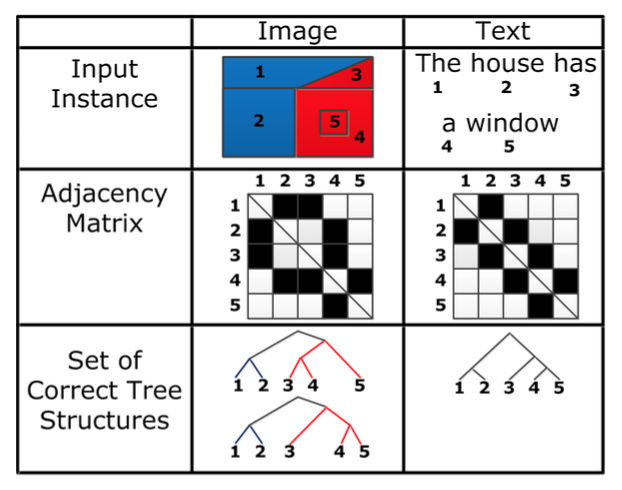
\includegraphics[width=2.1in]{images/fig3.png}   
		\end{center}   
		\caption{Illustrations of the RNN training inputs}
	\end{figure}
	\column{0.6\textwidth} 
	\begin{itemize}
	\item Goal : Learn a function $ f:\textit{X}\rightarrow\textit{Y} $
	\item Input $ x $ consists of two parts:
		\begin{enumerate}
		\item A set of activation vectors ${a_1, \dots, a_{N_{segs}}}$
		\item A symmetric adjacency matrix $ A $
		\end{enumerate}
	\end{itemize}
	\end{columns}
}
\frame
{
	\frametitle{Max-Margin Estimation}
	\begin{itemize}
		\item Define a structured margin loss $\Delta(x,l,\hat{y})$ similar to \textit{Taskar et al., 2004}
		\begin{Definition}
		$$ \Delta(x,l, \hat{y}) = \kappa \sum_{d \in \textbf{N}(\hat{y})} \textbf{1}\{\textit{subTree}(d) \notin Y(x,l)\}$$
		\end{Definition}
		\item The loss should be increased - when a segment merges with another one of a different label before merging with all its neighbors of the same label. 
		\item Formulated by checking whether the sub-tree $\textit{subTree}(d)$ underneath a nonterminal node $d$ 
		in $\hat{y}$ appears in any of the ground truth trees of $Y(x,l)$
	\end{itemize}
}
\frame
{
	\begin{itemize}
		\item Search for a function $ f $ with small expected loss on unseen inputs:
		$$ f_{\theta}(x) = \argmax_{\hat{y}\in\tau(x)} s(\text{RNN}(\theta, x, \hat{y}))$$
		where $\theta$ are all the parameters to cpompute a score $ s $ with an RNN and $ \tau(x) $
		denotes the set of all possible trees that can be constructed from an input x. 
		\item Margin constraints (score of the highest scoring correct tree $y_i$ to be larger up to a margin defined by the loss $ \Delta $)
		$$ s(\text(RNN)(\theta, x_i, y_i)) \geq s(\text{RNN}(\theta, x_i, \hat{y})) + \Delta(x_i, l_i, \hat{y})$$
	\end{itemize}
}
\frame
{
	\begin{itemize}
		\item Regularized risk function :
	\end{itemize}
		$$ J(\theta) = \frac{1}{N}\sum_{i=1}^N r_i(\theta) + \frac{\lambda}{2}||\theta||^2 \; where$$
		$$ r_i(\theta) = \max_{\hat{y}\in\tau(x_i)} s(\text{RNN}(\theta, x, \hat{y}) + \Delta(x_i, l_i, \hat{y})) - 
		\max_{y_i \in Y_{(x_i, l_i)}} (s\text{RNN}(\theta, x_i, y_i)) $$

	\begin{itemize}
		\item Minimize this objective $\rightarrow$ maximizes the correct tree's score and minimizes (up to a margin) 
		the score of the highest scoring but incorrect tree. 
	\end{itemize}
}
\frame
{
	\frametitle{Greedy Structure Prediction of RNNs}
	\begin{itemize}
		\item No efficient algorithms for RNN setting and $\exists$ exponentially 
		many possible parse trees $\rightarrow$ greedy approximation
		\item Find the pairs of neighboring segments and adds their activations to a set of potential child node pairs:
		$$ C = {[a_i, a_j]: A(i,j) = 1} $$
	\end{itemize}
}
\frame
{
	\begin{columns}
	\column{0.5\textwidth}
	\begin{figure}[ht]  
		\begin{center}
			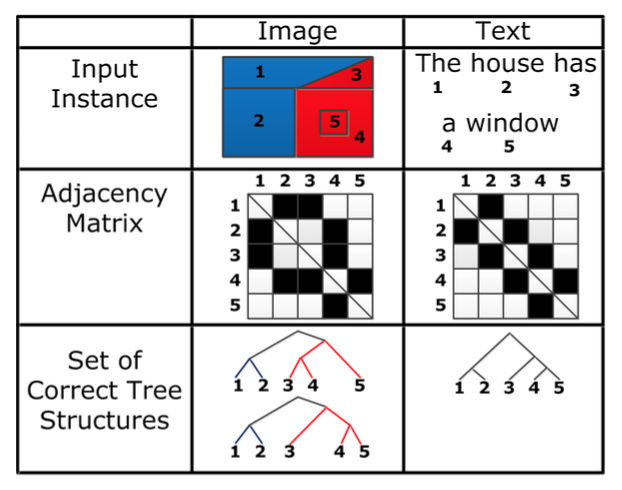
\includegraphics[width=2.1in]{images/fig3.png}   
		\end{center}   
	\end{figure}
	\column{0.6\textwidth} 
	\begin{itemize}
		\item For example :
		$$ C = \{[a_1, a_2], [a_1, a_3], [a_2, a_1], $$ 
		$$ [a_2, a_4], \dots  [a_4,a_5], [a_5, a_4]\} $$
	\end{itemize}
	\end{columns}
}
\frame
{
	\begin{columns}
	\column{0.4\textwidth}
	\begin{figure}[ht]  
		\begin{center}
			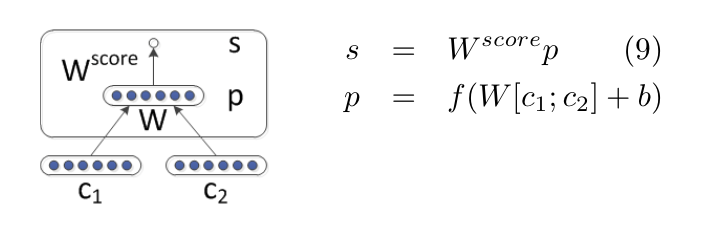
\includegraphics[width=2.2in]{images/fig4.png}   
		\end{center}   
	\end{figure}
	\column{0.6\textwidth} 
	\begin{itemize}
		\item The network computes the potential 
		parent representation in recursive way for the possible child nodes as $ \textit{p} $
		\item Local score can be calculated using a row vector 
		$ W^{score} \in \mathbb{R}^{1\times n} $
	\end{itemize}
	\end{columns}
}
\frame
{
	\begin{itemize}
		\item After computing the scores for all pairs of neighboring segments, 
		the algorithm selects the pair received the highest score. 
		\item Let the score $s_{ij}$ be the highest score
		\begin{enumerate}
			\item Remove $[a_i, a_j] $ from $C$ as well as all other pairs with 
			either $a_i$ or $a_j$ in them. 
			\item Update the adjacency matrix reflecting the new segment having the neighbors of both child segments
			\item Add potential new child pairs to $C$:
			$$ C = C - \{[a_i,a_j]\} - \{[a_j, a_i]\} $$
			$ C = C \cup \{[p_{(i,j)}, a_k]: a_k $ has boundary with $i$ or $j\}$
		\end{enumerate}
	\end{itemize}
}
\frame
{
	\begin{columns}
	\column{0.45\textwidth}
	\begin{figure}[ht]  
		\begin{center}
			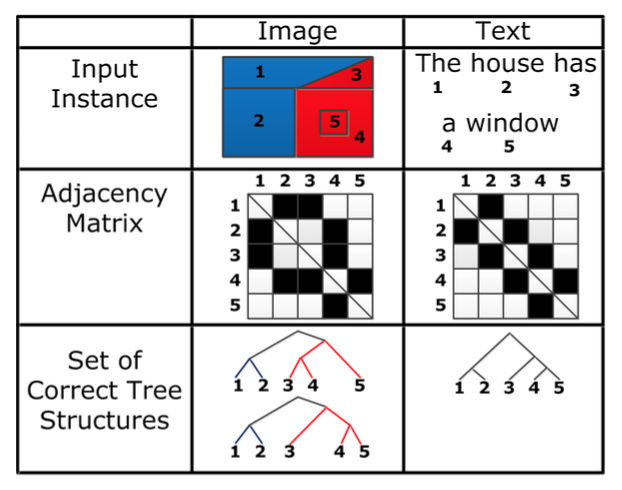
\includegraphics[width=2.in]{images/fig3.png}   
		\end{center}   
	\end{figure}
	\column{0.73\textwidth} 
	\begin{itemize}
		\item For example, if we merge $[a_4, a_5]$ then 
		$$ C = \{[a_1, a_2], [a_1, a_3], [a_2, a_1], [a_2, p_{(4,5)}], $$
		$$ [a_3, a_1], [a_3, p_{(4,5)}], [p_{(4,5)}, a_2], [p_{(4,5)}, a_3]\} $$
	\end{itemize}
	\end{columns}
}
\subsection{Learning}
\frame
{
}
\section{Experimental Results}
\subsection{Scene Understanding: Segmentation and Annotation}
\frame
{
  \frametitle{Parsing Natural Scene Images}
  \begin{columns}
  \column{0.5\textwidth}
  \begin{figure}[ht]  
	  \begin{center}
		  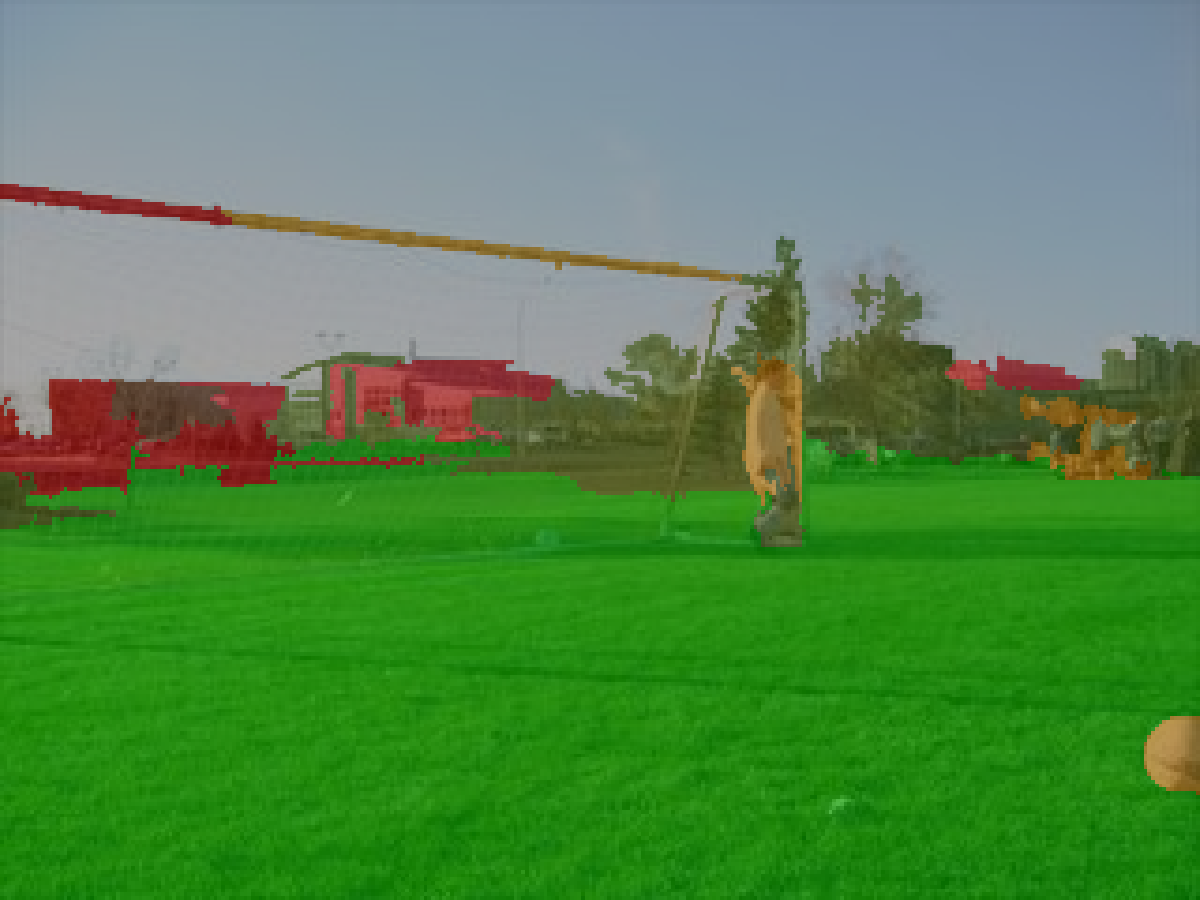
\includegraphics[width=2.1in]{images/ex1_ext.png}   
	  \end{center}   
  \end{figure}
  \column{0.5\textwidth} 
  \begin{figure}[ht]
	  \begin{center}
		  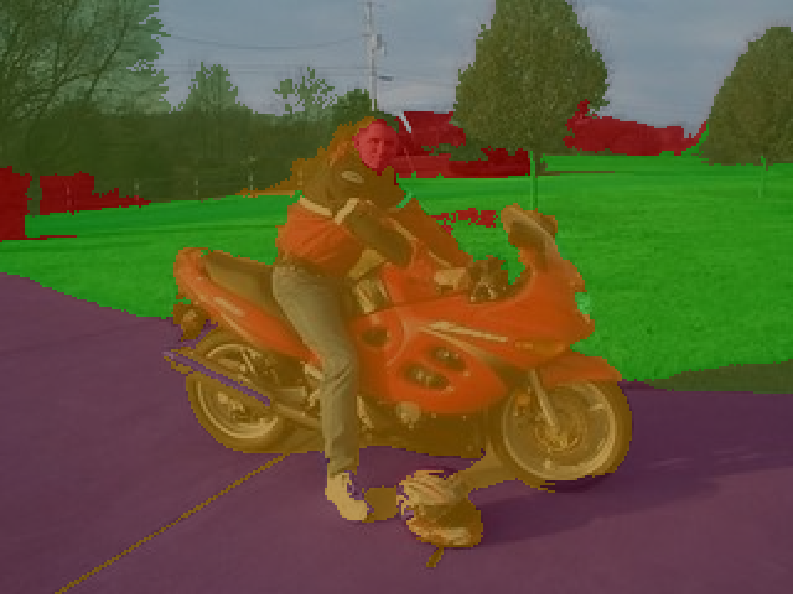
\includegraphics[width=2.1in]{images/ex1_ext2.png} 
	  \end{center}
  \end{figure}
  \end{columns}
}
\subsection{Scene Classification}
\frame
{
}
\subsection{Supervised Text Parsing}
\frame
{
}
\end{document}
